\documentclass[border=3pt,tikz]{standalone}
\usepackage{amsmath}
\usepackage{tikz}
\usepackage{tikz-3dplot}
\usepackage{physics}
\tikzset{>=latex} % for LaTeX arrow head
\usepackage{xcolor}
\usepackage{amsmath}
\usetikzlibrary{calc}
\colorlet{myblue}{black!40!blue}
\colorlet{myred}{black!40!red}
\colorlet{mygreen}{green!50!black}
\colorlet{darkorange}{orange!90!black}
\colorlet{EVcol}{orange!80!black!60}
\colorlet{myviolet}{violet!90}
\usetikzlibrary{calc}
\usetikzlibrary{arrows.meta} % for arrow size
\begin{document}
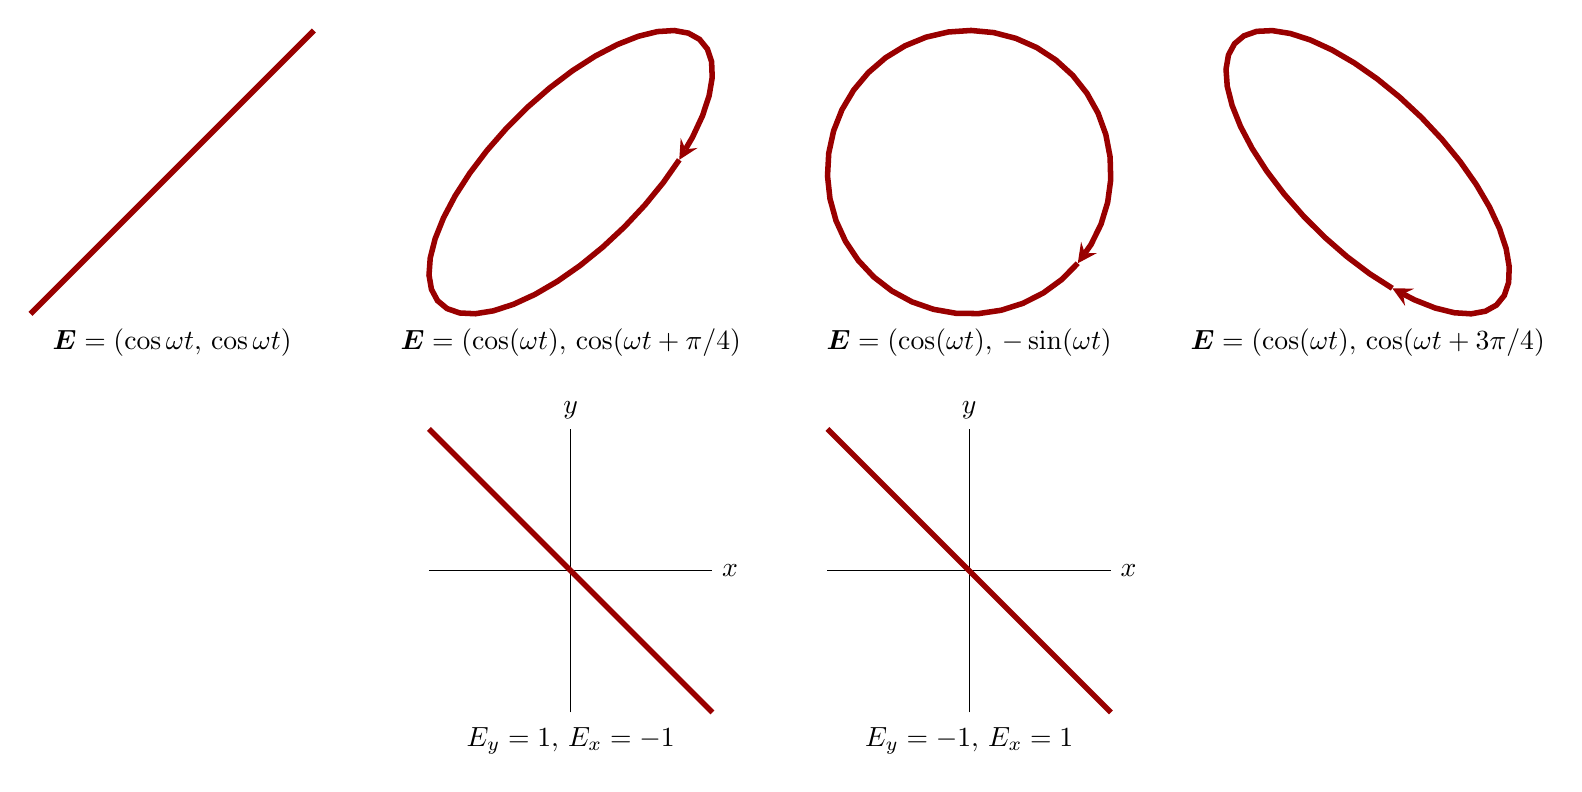
\begin{tikzpicture}[scale=1.8, rotate=0]
    \begin{scope}  
        \draw [line width=2, myred] (-1, -1) -- (1, 1);
        \node [] at (0, -1.2) {$\boldsymbol{E}=(\cos \omega t,\, \cos \omega t)$};
    \end{scope}
    \begin{scope} [xshift=80]
        \draw [myred, line width=2,  domain=40:400, samples=40, -stealth] plot ({cos(\x)}, {cos(\x+45)} );
        
        \node [] at (0, -1.2) {$\boldsymbol{E}=(\cos (\omega t),\, \cos(\omega t+\pi/4)$};
    \end{scope}
    \begin{scope} [xshift=160]
        \draw [myred, line width=2,  domain=40:400, samples=40, -stealth] plot ({cos(\x)}, {-sin(\x)} );
        \node [] at (0, -1.2) {$\boldsymbol{E}=(\cos (\omega t),\, -\sin(\omega t)$};
    \end{scope}
    \begin{scope} [xshift=240] 
        \draw [myred, line width=2,  domain=80:440, samples=40, -stealth] plot ({cos(\x)}, {cos(\x+135)} );
        
        \node [] at (0, -1.2) {$\boldsymbol{E}=(\cos (\omega t),\, \cos(\omega t+3\pi/4)$};
    \end{scope}
    \begin{scope} [xshift=80, yshift=-80]
        \draw (-1, 0) -- (1, 0) node [right] {$x$};
        \draw (0, -1) -- (0, 1) node [above] {$y$};
        \draw [line width=2, myred] (-1, 1) -- (1, -1);
        \node [] at (0, -1.2) {$E_y=1,\, E_x=-1$};
    \end{scope}
    \begin{scope} [xshift=160, yshift=-80]
        \draw (-1, 0) -- (1, 0) node [right] {$x$};
        \draw (0, -1) -- (0, 1) node [above] {$y$};
        \draw [line width=2, myred] (-1, 1) -- (1, -1);
        \node [] at (0, -1.2) {$E_y=-1,\, E_x=1$};
    \end{scope}
  


\end{tikzpicture}
\end{document}